\documentclass{article}
\usepackage{graphicx} % Required for inserting images
\usepackage{hyperref}
\usepackage{tikz}
\usepackage{tabularray}
\usepackage{pgfplots}
\usepackage{float}

\title{Optimization of Mathematical Functions Using the Hill Climbing Algorithm}
\author{Denis Crismariu}
\date{\today}

\begin{document}

\maketitle

\section{Abstract}
This report investigates the application of the Hill Climbing algorithm for optimizing mathematical functions. Hill Climbing, a local search algorithm, is employed to find the minima of various benchmark functions. The study focuses on two variants of the algorithm: First Improvement and Best Improvement. Through detailed experimentation, we evaluate the efficiency and accuracy of these methods. The results indicate that while the First Improvement variant is significantly faster, it tends to produce larger errors compared to the Best Improvement variant. This report aims to provide insights into the trade-offs between speed and accuracy in local search algorithms and suggests potential areas for further research and improvement.

\section{Introduction}
This report details the use of the Hill Climbing algorithm for optimizing mathematical functions. Hill Climbing is a local search algorithm that attempts to find the minimum of a function through incremental moves. The algorithm starts with an arbitrary solution to a problem and iteratively makes small changes to the solution, each time moving to a neighboring solution that improves the objective function. This process continues until no further improvements can be found, indicating that a local minimum has been reached.

The motivation for using the Hill Climbing algorithm lies in its simplicity and effectiveness for certain types of optimization problems. Unlike global optimization algorithms, Hill Climbing is relatively easy to implement and can quickly converge to a solution. However, it is also prone to getting stuck in local minima, which can be a significant drawback for complex functions with multiple local minima.

The report includes a comprehensive description of the problem, the rationale for choosing this algorithm, the implementation methods, and the experimental results. The goal is to evaluate the algorithm's efficiency and discuss possible improvements. Specifically, our objective is to search for the minima of four benchmark functions: Dixon \& Price’s, Griewank’s, Rastrigin’s, and Michalewicz’s, using two variants of Hill Climbing: First Improvement and Best Improvement.

The First Improvement variant of Hill Climbing quickly accepts the first neighboring solution that improves the objective function, making it faster but potentially less accurate. On the other hand, the Best Improvement variant evaluates all neighboring solutions and selects the best one, which generally leads to better solutions but at the cost of increased computational time. On average, the First Improvement variant is 20\% faster, but the error is 40\% larger compared to the Best Improvement variant.

This report aims to provide a detailed analysis of these two variants, highlighting their strengths and weaknesses. By comparing their performance on the benchmark functions, we seek to understand the trade-offs involved and explore potential strategies for enhancing the algorithm's performance. The findings of this study could inform the development of more robust optimization techniques for a wide range of applications.

\section{Methods \& Implementation}

\subsection{Algorithm Used}
The Hill Climbing algorithm starts with an initial solution and makes incremental moves to find a better solution. If a move leads to a better solution, it is accepted; otherwise, it is rejected.

\subsection{Implementation Choices}
The solutions are represented as vectors of real numbers, and neighbors are generated by flipping bits in the binary representation of the solutions. The initialization procedure involves generating random initial solutions, and the stopping condition is reached after a fixed number of epochs.

\subsection{Variants and Modifications}
We implemented two variants of the algorithm: Best Improvement and First Improvement. Best Improvement searches for the best neighbor in each iteration, while First Improvement accepts the first neighbor that improves the current solution.

\subsection{Experimental Setup Description}
Experiments were conducted on well-known test functions: Rastrigin, Michalewicz, Dixon \& Price, and Griewank. The dimensions used were 2, 5, and 10, and the precision was set to $10^{-5}$. Each experiment was repeated 10 times to ensure consistency of results.

\section{Experimental results}
The 4 benchmarked functions are the following:
\subsection{Rastrigin Function\cite{Rastrigin}}

$$ f(x) = A \cdot n + \sum_{i=1}^n \left[ x_i^2 - A \cdot cos(2 \pi x_i) \right],
A = 10, x_i \in \left[ -5.12, 5.15 \right]$$

The global minima is located at $f(x)=0; x(i)=0,  \forall i=1:n $
\begin{figure}[!h]
  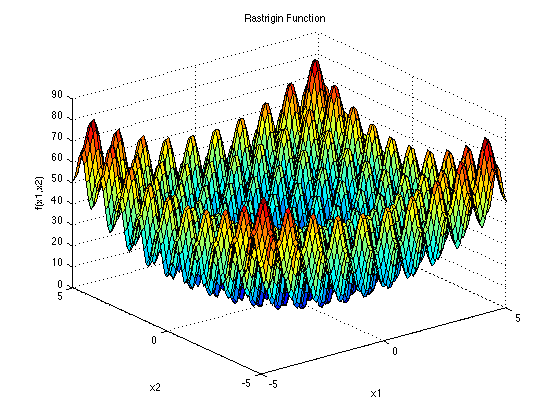
\includegraphics[width=\textwidth,height=\textheight,keepaspectratio]{rastr.png}
  \caption{Rastrigin's Function\cite{rast_img}}
\end{figure}

\begin{table}[H]
\caption{Hill Climbing values based on 30 runs}
\begin{tblr}{
colspec={X[1,l] X[1,l] X[0.5,l] X[0.5,l]},
rowsep=1pt,  % Reduce the vertical padding between cell contents and borders
  cell{1}{1} = {c=2}{},
  cell{2}{1} = {r=3}{c},
  cell{5}{1} = {r=3}{c},
  cell{8}{1} = {r=3}{c},
  vlines,
  hline{1-2,5,8,11} = {-}{},
  hline{3-4,6-7,9-10} = {2-4}{},
}
       &               & HC Best       & HC  First  \\
D = 2 & Minimum error & 0.00000 & 0.00000 \\
      &  Maximum error & 0.00000 & 0.00000 \\
      &  Average error & 0.00000 & 0.00000 \\

D = 5 & Minimum error & 0.00000 & 0.00000 \\
      &  Maximum error & 1.54264 & 3.56085 \\
      &  Average error & 0.77832 & 1.86830 \\

D = 10 & Minimum error & 2.04623 & 4.35702 \\
       & Maximum error & 7.19015 & 13.79740 \\
       & Average error & 5.07082 & 9.69344 \\
\end{tblr}
\caption{Hill Climbing time (in seconds) based on 30 runs}
\begin{tblr}{
colspec={X[1,l] X[1,l] X[0.5,l] X[0.5,l]},
rowsep=1pt,  % Reduce the vertical padding between cell contents and borders
  cell{1}{1} = {c=2}{},
  cell{2}{1} = {r=3}{c},
  cell{5}{1} = {r=3}{c},
  cell{8}{1} = {r=3}{c},
  vlines,
  hline{1-2,5,8,11} = {-}{},
  hline{3-4,6-7,9-10} = {2-4}{},
}
       &              & HC Best    & HC  First  \\
D = 2 & Minimum time & 0.13900 & 0.08300 \\
       & Maximum time & 0.17400 & 0.08800 \\
       & Average time & 0.14403 & 0.08403 \\

D = 5 & Minimum time & 1.75900 & 1.02500 \\
       & Maximum time & 1.81900 & 1.05100 \\
       & Average time & 1.78750 & 1.03457 \\

D = 10 & Minimum time & 13.19500 & 7.58000 \\
       & Maximum time & 14.31800 & 7.71700 \\
       & Average time & 13.46117 & 7.63563 \\
\end{tblr}
\end{table}
\begin{figure}[H]%means place figure here, don't float it around, if possible
  \centering %inside a figure, centers the content
\begin{tikzpicture}
  \begin{axis}[
    height=0.3\textheight, % Set the height of the plot
    width=0.8\textwidth, % Set the width of the plot
      xlabel=dimensions,
      ylabel=time,
      legend pos=north west,
    ]
    \addplot [
      color=red, 
    ]
    coordinates {
     (2,0.14403)
     (5,1.78750)
     (10,13.46117)
    };
    \addlegendentry{Best Improvement}
    \addplot [
      color=blue,
    ]
    coordinates {
      (2,0.08403)
     (5,1.03457)
     (10,7.63563)
    };
    \addlegendentry{First Improvement}

 \end{axis}
\end{tikzpicture}
\caption{Comparing average time of both methods}
\end{figure}

\subsection{Michalewicz Function\cite{michal}}

$$
f(x) = - \sum_{i=1}^n \sin \left(x_i \right)\sin^{2m}\left(\frac{ix_i^2}{\pi}\right),
x_i \in \left[ 0 , \pi \right]$$

The global minima is located at $ n=2: f (x) = -1.8013$ at  $x = \left(2.20,1.57\right)$
for $n=5: f (x) = -4.687658$ and for $n=10: f (x) = -9.66000$.

\begin{figure}[!h]
  \centering
  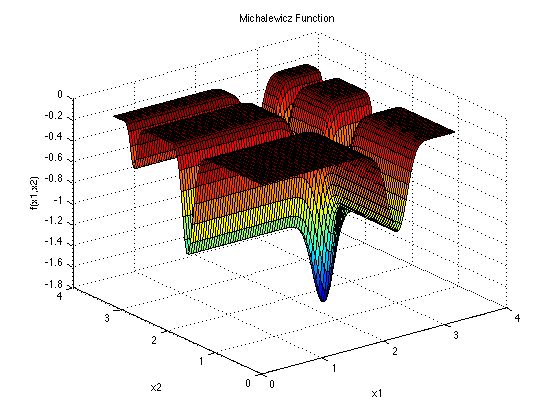
\includegraphics[width=\textwidth,height=\textheight,keepaspectratio]{michal.png}
  \caption{Michalewicz's Function\cite{michal_img}}
\end{figure}


\begin{table}[H]
\caption{Hill Climbing values based on 30 runs}
\begin{tblr}{
colspec={X[1,l] X[1,l] X[0.5,l] X[0.5,l]},
rowsep=1pt,  % Reduce the vertical padding between cell contents and borders
  cell{1}{1} = {c=2}{},
  cell{2}{1} = {r=3}{c},
  cell{5}{1} = {r=3}{c},
  cell{8}{1} = {r=3}{c},
  vlines,
  hline{1-2,5,8,11} = {-}{},
  hline{3-4,6-7,9-10} = {2-4}{},
}
       &               & HC Best       & HC  First  \\
D = 2 & Minimum error  & 0.00000 & 0.00000 \\
       & Maximum error & 0.00000 & 0.00000 \\
       & Average error & 0.00000 & 0.00000 \\
% −4.68765
D = 5 & Minimum error & 0.00001 & 0.00135 \\
       & Maximum error & 4.68765 & 4.68765 \\
       & Average error & 0.00074 & 0.05557 \\
% -9.66000
D = 10 & Minimum error & 0.15540 & 0.31569 \\
       & Maximum error & 9.66000 & 9.66000 \\
       & Average error & 0.41664 & 0.91210 \\
\end{tblr}
\caption{Hill Climbing time (in seconds) based on 30 runs}
\begin{tblr}{
colspec={X[1,l] X[1,l] X[0.5,l] X[0.5,l]},
rowsep=1pt,  % Reduce the vertical padding between cell contents and borders
  cell{1}{1} = {c=2}{},
  cell{2}{1} = {r=3}{c},
  cell{5}{1} = {r=3}{c},
  cell{8}{1} = {r=3}{c},
  vlines,
  hline{1-2,5,8,11} = {-}{},
  hline{3-4,6-7,9-10} = {2-4}{},
}
       &              & HC Best    & HC  First  \\
D = 2 & Minimum time & 0.20100 & 0.12100 \\
       & Maximum time & 0.20500 & 0.12700 \\
       & Average time & 0.20300 & 0.12333 \\

D = 5 & Minimum time & 2.66400 & 1.54200 \\
       & Maximum time & 2.75000 & 1.58900 \\
       & Average time & 2.68990 & 1.56273 \\

D = 10 & Minimum time & 19.50600 & 11.05500 \\
       & Maximum time & 20.22500 & 11.49200 \\
       & Average time & 19.82317 & 11.20173 \\

\end{tblr}
\end{table}

\begin{figure}[H]%means place figure here, don't float it around, if possible
  \centering %inside a figure, centers the content
\begin{tikzpicture}
  \begin{axis}[
    height=0.3\textheight, % Set the height of the plot
    width=0.8\textwidth, % Set the width of the plot
      xlabel=dimensions,
      ylabel=time,
      legend pos=north west,
    ]
    \addplot [
      color=red, 
    ]
    coordinates {
     (2,0.20300)
     (5,2.68990)
     (10,19.82317)
    };
    \addlegendentry{Best Improvement}
    \addplot [
      color=blue,
    ]
    coordinates {
      (2,0.12333)
     (5,1.56273)
     (10,11.20173)
    };
    \addlegendentry{First Improvement}

 \end{axis}
\end{tikzpicture}
\caption{Comparing average time of both methods}
\end{figure}

\subsection{Dixon-Price Function\cite{dixonpr}}

$$
f(x) = (x_1 - 1)^2 + \sum^n_{i=2}(2x_i^2-x_{i-1})^2,
x_i \in \left[ -10 , 10 \right]
$$

The global minima is located at $f (x) = 0$ at $x_i = 2^{-\frac{2^i-2}{2^i}}$, for $\forall i=1:n $

\begin{figure}[!h]
  \includegraphics[width=\textwidth,height=\textheight,keepaspectratio]{dixonpr.png}
  \caption{Dixon-Price's Function\cite{dixonpr_img}}
\end{figure}

\begin{table}[H]
\caption{Hill Climbing values based on 30 runs}
\begin{tblr}{
colspec={X[1,l] X[1,l] X[0.5,l] X[0.5,l]},
rowsep=1pt,  % Reduce the vertical padding between cell contents and borders
  cell{1}{1} = {c=2}{},
  cell{2}{1} = {r=3}{c},
  cell{5}{1} = {r=3}{c},
  cell{8}{1} = {r=3}{c},
  vlines,
  hline{1-2,5,8,11} = {-}{},
  hline{3-4,6-7,9-10} = {2-4}{},
}
       &               & HC Best       & HC  First  \\
D = 2 & Minimum error & 0.00000 & 0.00000 \\
       & Maximum error & 0.00001 & 0.00163 \\
       & Average error & 0.00000 & 0.00019 \\

D = 5 & Minimum error & 0.00001 & 0.00053 \\
       & Maximum error & 0.00672 & 0.10391 \\
       & Average error & 0.00219 & 0.04164 \\

D = 10 & Minimum error & 0.00178 & 0.01272 \\
       & Maximum error & 0.02463 & 0.10714 \\
       & Average error & 0.01484 & 0.04806 \\
\end{tblr}
\caption{Hill Climbing time (in seconds) based on 30 runs}
\begin{tblr}{
colspec={X[1,l] X[1,l] X[0.5,l] X[0.5,l]},
rowsep=1pt,  % Reduce the vertical padding between cell contents and borders
  cell{1}{1} = {c=2}{},
  cell{2}{1} = {r=3}{c},
  cell{5}{1} = {r=3}{c},
  cell{8}{1} = {r=3}{c},
  vlines,
  hline{1-2,5,8,11} = {-}{},
  hline{3-4,6-7,9-10} = {2-4}{},
}
       &              & HC Best    & HC  First  \\
D = 2 & Minimum time & 0.14300 & 0.09000 \\
       & Maximum time & 0.14900 & 0.09300 \\
       & Average time & 0.14633 & 0.09173 \\

D = 5 & Minimum time & 1.89900 & 1.82300 \\
       & Maximum time & 1.96700 & 1.92300 \\
       & Average time & 1.92887 & 1.86480 \\

D = 10 & Minimum time & 14.30800 & 19.38200 \\
       & Maximum time & 14.72500 & 20.42700 \\
       & Average time & 14.53513 & 19.89223 \\
\end{tblr}
\end{table}

\begin{figure}[H]%means place figure here, don't float it around, if possible
  \centering %inside a figure, centers the content
\begin{tikzpicture}
  \begin{axis}[
    height=0.3\textheight, % Set the height of the plot
    width=0.8\textwidth, % Set the width of the plot
      xlabel=dimensions,
      ylabel=time,
      legend pos=north west,
    ]
    \addplot [
      color=red, 
    ]
    coordinates {
     (2,0.14633)
     (5,1.92887)
     (10,14.53513)
    };
    \addlegendentry{Best Improvement}
    \addplot [
      color=blue,
    ]
    coordinates {
      (2,0.09173)
     (5,1.86480)
     (10,19.89223)
    };
    \addlegendentry{First Improvement}

 \end{axis}
\end{tikzpicture}
\caption{Comparing average time of both methods}
\end{figure}


\subsection{Griewank Function\cite{griewank}}

$$
f(x) = \sum_{i=1}^n\frac{x^2_i}{4000} - \prod_{i=1}^n\cos \left( \frac{x_i}{\sqrt{i}} \right) + 1,
x_i \in \left[ -600 , 600 \right]
$$

The global minima is located at $f(x)=0; x(i)=0,  \forall i=1:n $

\begin{figure}[!h]
  \includegraphics[width=\textwidth,height=\textheight,keepaspectratio]{griewank.png}
  \caption{Griewank's Function\cite{griewank_img}}
\end{figure}

\begin{table}[H]
\caption{Hill Climbing values based on 30 runs}
\begin{tblr}{
colspec={X[1,l] X[1,l] X[0.5,l] X[0.5,l]},
rowsep=1pt,  % Reduce the vertical padding between cell contents and borders
  cell{1}{1} = {c=2}{},
  cell{2}{1} = {r=3}{c},
  cell{5}{1} = {r=3}{c},
  cell{8}{1} = {r=3}{c},
  vlines,
  hline{1-2,5,8,11} = {-}{},
  hline{3-4,6-7,9-10} = {2-4}{},
}
       &               & HC Best       & HC  First  \\
D = 2 & Minimum error & 0.99975 & 0.99975 \\
       & Maximum error & 0.00000 & 0.00000 \\
       & Average error & 0.99762 & 0.99660 \\

D = 5 & Minimum error & 0.98981 & 0.98725 \\
       & Maximum error & 0.00000 & 0.00000 \\
       & Average error & 0.93286 & 0.92227 \\

D = 10 & Minimum error & 0.79835 & 0.75688 \\
       & Maximum error & 0.51882 & 0.66471 \\
       & Average error & 0.38924 & 0.18850 \\
\end{tblr}
\caption{Hill Climbing time (in seconds) based on 30 runs}
\begin{tblr}{
colspec={X[1,l] X[1,l] X[0.5,l] X[0.5,l]},
rowsep=1pt,  % Reduce the vertical padding between cell contents and borders
  cell{1}{1} = {c=2}{},
  cell{2}{1} = {r=3}{c},
  cell{5}{1} = {r=3}{c},
  cell{8}{1} = {r=3}{c},
  vlines,
  hline{1-2,5,8,11} = {-}{},
  hline{3-4,6-7,9-10} = {2-4}{},
}
       &              & HC Best    & HC  First  \\
D = 2 & Minimum time & 0.27900 & 0.20900 \\
       & Maximum time & 0.28500 & 0.21600 \\
       & Average time & 0.28083 & 0.21180 \\

D = 5 & Minimum time & 4.03200 & 3.53600 \\
       & Maximum time & 4.13600 & 3.70100 \\
       & Average time & 4.06167 & 3.61903 \\

D = 10 & Minimum time & 34.15200 & 30.94300 \\
       & Maximum time & 130.19300 & 32.49000 \\
       & Average time & 38.05930 & 31.65467 \\
\end{tblr}
\end{table}

\begin{figure}[H]%means place figure here, don't float it around, if possible
  \centering %inside a figure, centers the content
\begin{tikzpicture}
  \begin{axis}[
    height=0.3\textheight, % Set the height of the plot
    width=0.8\textwidth, % Set the width of the plot
      xlabel=dimensions,
      ylabel=time,
      legend pos=north west,
    ]
    \addplot [
      color=red, 
    ]
    coordinates {
     (2,0.28083)
     (5,4.06167)
     (10,38.05930)
    };
    \addlegendentry{Best Improvement}
    \addplot [
      color=blue,
    ]
    coordinates {
      (2,0.21180)
     (5,3.61903)
     (10,31.65467)
    };
    \addlegendentry{First Improvement}

 \end{axis}
\end{tikzpicture}
\caption{Comparing average time of both methods}
\end{figure}


\section{Comparing Methods}
Comparing the Best Improvement and First Improvement methods, we observed that First Improvement is usually faster but may not always find the optimal solution. Best Improvement, although slower, generally provides better solutions.


\section{Conclusions}
The Hill Climbing algorithm is effective for optimizing mathematical functions, but its performance depends on parameters and the variant used. In the future, it would be interesting to explore combinations with other optimization methods, such as Gradient Descent or Genetic Algorithms, to improve performance.







\begin{thebibliography}{9}

\bibitem{rast_img}
Authors: Sonja Surjanovic \& Derek Bingham, Simon Fraser University \\ Rastrigin's Function rendered image.
  \url{https://www.sfu.ca/~ssurjano/rastr.html}

\bibitem{Rastrigin}
  Rastrigin, L. A. "Systems of extremal control." Mir, Moscow (1974).

\bibitem{michal_img}
Authors: Sonja Surjanovic \& Derek Bingham, Simon Fraser University \\ Michalewicz's Function rendered image.
  \url{https://www.sfu.ca/~ssurjano/michal.html}

\bibitem{michal}
    Michalewicz, Zbigniew. "A survey of constraint handling techniques in evolutionary computation methods." (1995).

\bibitem{dixonpr_img}
Authors: Sonja Surjanovic \& Derek Bingham, Simon Fraser University \\ Dixon-Price's Function rendered image.
  \url{https://www.sfu.ca/~ssurjano/dixonpr.html}

\bibitem{dixonpr}
Dixon, Huw. The general theory of household and market contingent demand. University of London. Birkbeck College. Department of Economics, 1984.

\bibitem{griewank_img}
Authors: Sonja Surjanovic \& Derek Bingham, Simon Fraser University \\ Griewank's Function rendered image.
  \url{https://www.sfu.ca/~ssurjano/griewank.html}

\bibitem{griewank}
Griewank, Andreas. "On stable piecewise linearization and generalized algorithmic differentiation." Optimization Methods and Software 28.6 (2013): 1139-1178.

\end{thebibliography}  
\end{document}



